\documentclass[a4paper]{article}
\usepackage{a4wide,graphicx,color}
\usepackage{natbib}
\usepackage{hyperref}

\definecolor{Red}{rgb}{0.7,0,0}
\definecolor{Blue}{rgb}{0,0,0.8}


\usepackage{c:/Programmer/R/R-2.2.1/share/texmf/Sweave}
\begin{document}

%\VignetteIndexEntry{Bioassay analysis using R}
%\VignetteKeywords{effective dosage, multiple dose response curves, non-linear regression}
%\VignettePackage{drc}

\title{Bioassay Analysis using \textbf{R}}
\author{\hfill Christian Ritz$^\dag$ \hfill Jens C. Streibig$^\ddag$ \hfill \hfill \\
\dag {\it \small Derpartment of Natural Sciences, Royal Veterinary and Agricultural University, Denmark}\\
\ddag {\it \small Department of Agricultural Sciences, Royal Veterinary and Agricultural University, Denmark}}
%\date{}

\maketitle

%% an abstract and keywords
\abstract{
We describe an add-on package for the language and environment \textbf{R} which allows
simultaneous fitting of several non-linear regression models. The focus is on analysis of dose response curves, but the functionality is applicable
to arbitrary non-linear regression models. Features of the package is illustrated in examples.
}
\\
\\
\emph{Keywords}: dose response data, multiple curves, non-linear regression


\section{Introduction} 

Bioassays are experiments with biologically active compounds.
In herbicide selectivity studies it is
common to run suites of bioassays with dose response curves for
different plant species and/or different herbicide preparations.
The same principles apply to the study of compounds in toxicology
and pharmacology. In herbicide research and development, potencies of compounds usually are
compared at some \emph{a priori} response
levels, say 50\% reduction (ED50) in biomass or other response
variables. For example, ED10 denotes 10\% effect, that is 90\% of the untreated control.
To describe herbicide selectivity we compare
tolerance of crops, say ED10, and sensitivity of
weeds, say ED90. These ways of comparing compound potencies and/or
species sensitivity also are widely used in ecotoxicology of
xenobiotics.

Therefore, it is relevant to develop software which is capable of
carrying out simultaneous non-linear regression analysis on
several bioassays. In this paper we will demonstrate the use of
the software package \verb+drc+ for analysis of multiple
dose response curves. The functions in \verb+drc+ provide a convenient means for specifying
models, controlling the minimization and retrieving relevant
results, including comparisons of parameters of interest.

The package \verb+drc+ is an add-on package
for the language and environment \textbf{R} \citep{r-lang} which
is open source and freely available (see
http://www.R-project.org). \textbf{R} is an implementation of the
language S.

The approach taken is to illustrate the functionality through
several examples, where the function calls in \textbf{R} and the resulting
output are interwoven into explanatory text. In this manner we present
applications of the main functions contained in \verb+drc+. We do
not give an exhaustive description of the numerous facilities in
\verb+drc+. However, we wish to emphasize that various non-linear regression
models can be fit using \verb+drc+.

Sections~\ref{sec:2} introduces the relevant statistical models and some aspects related to the parameters in the models. 
An overview of the package \verb+drc+ is given in section~\ref{sec:3}.
In sections~\ref{sec:4}, \ref{sec:5}, \ref{sec:6} and \ref{sec:7} we illustrate some of the features 
and functionality of \verb+drc+ for various aspects of fitting non-linear regression models with emphasis on bioassay analysis.

%######################################################
%######################################################
%######################################################

\section{Non-linear regression models for bioassay data} \label{sec:2}

We consider a suite of $n$ dose response curves and we assume
that for each dose response curve the response follows a non-linear curve
specified by the function $f$, which is known apart from a
parameter vector that may be different for different curves. Thus, the model for the \emph{i}th dose response
curve is

\[ 
y_{ij} = f (x_{ij}, \alpha_i) + \varepsilon_{ij} \qquad j=1, \ldots, m_i, \qquad i=1, \ldots, n, 
\]
where $x_{ij}$ denotes the $j$th dose value in the $i$th dose response curve and $y_{ij}$ is the resulting response value, $\alpha_i$ is the 
unknown parameter vector for dose response curve $i$ and
$\varepsilon_{ij}$ is the measurement error for the response $y_{ij}$. The measurement
errors $\varepsilon_{11}, \ldots, \varepsilon_{n m_n}$ are
assumed mutually independent and normally distributed $N(0,
\sigma^2)$. In particular, all observations have the same variance
(variance homogeneity).

The parameters are estimated using non-linear least squares which
amounts to minimizing the sum of squares 

\[ 
\sum_{i=1}^n \sum_{j=1}^{m_i} \big( y_{ij} - f (x_{ij}, \alpha_i) \big)^2 
\] 
with respect to the parameters $(\alpha_1, \ldots, \alpha_n)$.

\subsection{Commonly used models} \label{sec:2.1}

 
Two models for sigmoidal dose response curves are widely used: The logistic and Weibull models. We will briefly discuss these models. 
 
The four-parameter logistic function is given by the formula

\begin{equation} \label{l4}
f \big(x, (b,c,d,e) \big)=  c+\frac{d-c}{1+\exp \big\{b \big( \log(x)-\log(e) \big)  \big\}}
\end{equation}

\noindent with 4 parameters $b, c, d, e$. The parameter $e$ is also
denoted ED50 and it is the dose producing a response half-way
between the upper limit, $d$, and  lower limit, $c$. The parameter $b$ denotes
the relative slope around $e$.  The interpretation of the parameters is discussed by \citet{streibig&rudemo&jensen:1993}. The logistic function
is symmetric around $e$.
The three-parameter logistic model with the lower limit equal to 0 has the form:

\[ 
f \big(x, (b,d,e) \big)= \frac{d}{1+\exp \big\{b \big( \log(x)-\log(e) \big)  \big\}}
\]
and the five-parameter logistic model \citep{finney:1979} is given
by the formula

\begin{equation} \label{l5}
f \big(x, (b,c,d,e,f) \big) = c+\frac{d-c}{\big(1+\exp \big\{b \big( \log(x)-\log(e) \big) \big\} \big)^f}.
\end{equation}
Letting the parameter $f$ be equal to 1 in (\ref{l5}) yields the four-parameter logistic model (\ref{l4}). 

The four-parameter Weibull model is given by the formula

\begin{equation} \label{w4}
f \big(x, (b,c,d,e) \big) = c+(d-c) \exp\{ -\exp\{ b(\log (x)- e)\}  \}.
\end{equation}
The parameters $c$ and $d$ are the lower and upper
limits, as for four-parameter logistic model, $b$ is
the relative slope around $e$, and the $e$ parameter is the logarithm of the inflection point. The Weibull model is not symmetric around any point.
The three-parameter Weibull model with the lower limit equal to 0 is then

\[
f \big(x, (b,d,e) \big) = d \exp\{ -\exp\{ b(\log (x)- e)\}  \}.
\]
Besides the Weibull model and the logistic model, Brain-Cousens' model \citep{brain&cousens:1989} is used in situations where \emph{hormesis} is present: 
For small doses the herbicide has the adverse effect resulting in response values above the level of the control group 
\citep{calabrese&baldwin:2001, calabrese&baldwin:2003}. Brain-Cousens model is obtained by modifying the four-parameter logistic model

\begin{equation} \label{bcl4}
f \big(x, (b,c,d,e) \big)=  c+\frac{d+fx-c}{1+\exp \big\{b \big( \log(x)-\log(e) \big)  \big\}}
\end{equation}
adding the linear term $fx$ in the numerator. Again we could also consider the modification where the lower limit is set equal to 0.
\\
\\
Notice that the $b$ and $e$ parameters are different in (\ref{l4}), (\ref{l5}), (\ref{w4}) and (\ref{bcl4}), respectively.
In this paper we assume that the response is a decreasing function of the dose (from maximum response to lower limit), corresponding to positive $b$, 
but the models also apply to situation where the response is increasing with the dose.


\subsection{Initial parameter values and self starter functions}

Contrary to linear regression, estimation of parameters in non-linear regression requires the specification of initial parameter values. The choice
of the values may influence on the convergence of the estimation algorithm, in the worst case yielding no convergence and in the best case convergence
in few iterations. 

For many non-linear functions it may be possible to obtain sensible initial parameter values using the interpretation of the parameters.
For the four-parameter logistic function this is done by using the maximum (initial value of $d$) and minimum (initial value of $c$) value of the $y$s and 
then making the transformation

\begin{equation}
\log\left(\frac{d-y}{y-c}\right)=b(\log(x)-\log(e)).
\end{equation}
Now linear regression can be used to obtain initial values of $b$ and $e$. The procedure described can be captured in a function which for a given data
set returns starting values. We will refer to such a function as a self starter function.
A similar approach can be used for the Weibull model and Brain-Cousens' model. For another example see section~\ref{sec:7}.


\subsection{Comparison of parameters} \label{sec:2.2}

Having several fitted dose response curves, it may be of interest to compare parameters across curves, for instance comparing lower limits for
different curves. 

Typically, in bioassay analysis, the main interest lies in comparing quantities that are functions of the parameters. The common approach has been 
to re-parameterize and 
re-fit the model for each function of interest \citep{schabenberger&tharp&kells&penner:1999}. This approach is relatively computer-intensive, 
requires some skill in manipulating mathematical expressions and moreover is vulnerable to lack of convergence of the
non-linear least squares algorithm, as the re-parameterization could result in strongly correlated parameters depending upon the distribution of
the responses between the lower and upper limits. Therefore we implement a single-model approach where a single model is fit and the delta method 
\citep[chap.~3]{vandervaart:1998}, is used to calculate approximate standard errors for functions of the parameters.

The quantities effective dosage (ED) and selectivity index (SI) are commonly used to compare different herbicides. Both ED and SI are functions of the
parameters: EDy is defined as the dose that yields a response which is (100-y)\% of the maximal response $d$ (a reduction of y\%). 
For instance, EDy can be expressed by means of the parameters $b$ and $e$ in the four-parameter logistic model

\[
\mbox{EDy} = e (y/(100 - y))^{1/b}.
\] 
The Weibull model yields a similar formula. For Brain-Cousens' model there are no closed-form solutions, but numerical methods can be applied; we
use the bisection method. SI(x,y) is the ratio between EDx for one curve and EDy for another curves. 

\[
\mbox{SI(x,y)} = \mbox{EDx} / \mbox{EDy}
\]
In section~\ref{sec:5} we will illustrate the interpretation of ED and SI based on an example. 


%######################################################
%######################################################
%######################################################

%\newpage
\section{About the package} \label{sec:3}

The \verb+drc+ package consists entirely of interpreted R lines. This paper describes version 0.8-1. The current version as well as future versions 
can be found at www.bioassay.dk.

The main function is \verb+multdrc+ which carries out the estimation of parameters and returns a model fit, an object of class 'drc'. The default 
optimisation method is a variant of the Newton algorithm, but this setting can be changed in \verb+multdrc+. The functions 
described in subsection~\ref{sec:2.1} are built-in in \verb+multdrc+ and available by specifying the \verb+fct+ argument. 
Table~\ref{sec3-table1} provides a list of some of the built-in functions available.

\begin{table}[!htbp]
\begin{center}
\begin{tabular}{|l|l|}
\hline
Function & Model\\
\hline
%\verb+mg4()+ & Modified four-parameter Weibull\\
\verb+l3()+ & Three-parameter logistic\\
\verb+l4()+ & Four-parameter logistic (default)\\
\verb+l5()+ & Five-parameter logistic\\
\verb+bcl3()+ & Brain-Cousens three-parameter logistic\\
\verb+bcl4()+ & Brain-Cousens four-parameter logistic\\
%\verb+ml4()+ & Modified four-parameter logistic\\
\verb+w3()+ & Three-parameter Weibull\\
\verb+w4()+ & Four-parameter Weibull\\
\hline
\end{tabular} \caption{Built-in functions in the package \texttt{drc}.} \label{sec3-table1}
\end{center} 
\end{table}

\noindent The default value is the four-parameter logistic model, that is \verb+l4()+ (which need not be specified). 
It is possible to specify initial parameter values manually, but as it may be difficult to guess at values of the parameters 
for the less experienced researcher, the built-in functions in \verb+drc+ have self starter functions. 
User-defined functions with a user-defined self starter function can be specified (see section~\ref{sec:7}). 

Once a model fit is obtained using \verb+multdrc+, the following methods are available for objects of class 'drc', for extracting information

\begin{itemize}
\item \verb+anova+: lack-of-fit test or test for reduction between two models
\item \verb+coef+: parameter estimates
\item \verb+fitted+: fitted values
\item \verb+logLik+ log likelihood value
\item \verb+plot+: plot of the fitted curves
\item \verb+residuals+: raw residuals
\item \verb+summary+: summary of the model fit
\item \verb+vcov+: estimated variance-covariance matrix
\end{itemize} 

In addition the function \verb+plotraw+ produces a plot of the observations, all curves in a single plot or a plot for each curve.
The functions \verb+compParm+, \verb+ED+ and \verb+SI+ provide comparisons of parameters, ED values and SI values, respectively. 
The functions \verb+ED+ and \verb+SI+ work with the built-in nonlinear functions. User-defined functions can also be made to work with \verb+ED+ 
and \verb+SI+, but it requires that they provide additional formulas for the calculation of ED values and their standard errors.
The function \verb+diagnostics+ supplies brief information about convergence of the estimation algorithm.



%######################################################
%######################################################
%######################################################

\newpage
\section{Fitting a single dose response curve} \label{sec:4}

To get started we need to load the package \verb+drc+. This is done using the \verb+library+ function

\begin{Schunk}
\begin{Sinput}
> library(drc)
\end{Sinput}
\begin{Soutput}
Loading required package: MASS
\end{Soutput}
\end{Schunk}
The data sets that we will use in this paper are all part of the package. In this section we use the data set \verb+FA+
consisting of a single dose response curve (use \verb+data(FA)+ to load the data set). The first 5 lines (rows) of the data set are 
displayed by typing \verb+FA[1:5,]+

\begin{Schunk}
\begin{Sinput}
> data(FA)
> FA[1:5, ]
\end{Sinput}
\begin{Soutput}
    MEANLR MM
1 7.580000  0
2 8.000000  0
3 8.328571  0
4 7.250000  0
5 7.375000  0
\end{Soutput}
\end{Schunk}
The variable \verb+MM+ is the dose of ferulic acid in mM and \verb+MEANLR+ is the root length of perennial ryegrass 
\citep{inderjit&streibig&olofsdotter:2002}.

As already mentioned the main function in \verb+drc+ for fitting dose response curves is \verb+multdrc+ which can be used to fit data from one or 
more dose response curves.
By default a four-parameter logistic model is fitted to the data. In order to fit this model to 
the data set \verb+FA+ we write 

\begin{Schunk}
\begin{Sinput}
> modelex1 <- multdrc(FA)
\end{Sinput}
\end{Schunk}
The argument to the function \verb+multdrc+ is a data frame 
which is a collection of columns of the same length, usually forming a data set or part of 
a data set. The above \textbf{R} call, \verb+multdrc(FA)+, produces no output. All relevant information of the fit of the model
to the data is stored in the object \verb+modelex1+. The package \verb+drc+ provides \emph{extractors} for extracting
various types of information from \verb+modelex1+. We will now introduce some of these extractors.

The \verb+anova+ function can be used to obtain a lack-of-fit test, comparing the four-parameter logistic model to a one-way ANOVA model

\begin{Schunk}
\begin{Sinput}
> anova(modelex1)
\end{Sinput}
\begin{Soutput}
Lack-of-fit test

              ModelDf    RSS Df F value p value
One-way ANOVA      17 5.1799                   
DRC model          20 5.4002  3  0.2411  0.8665
\end{Soutput}
\end{Schunk}
The test is not significant, implying that the four-parameter logistic model provides as good a fit as the one-way ANOVA.
A summary of the fit, including the type of model fitted, the parameter estimates and their
standard deviations, is obtained using the \verb+summary+ function

\begin{Schunk}
\begin{Sinput}
> summary(modelex1)
\end{Sinput}
\begin{Soutput}
A 'logistic' model was fitted.

Parameter estimates:

              Estimate Std. Error  t-value   p-value
b:(Intercept)  2.98183    0.46500  6.41249 2.960e-06
c:(Intercept)  0.48114    0.21221  2.26727    0.0346
d:(Intercept)  7.79306    0.18857 41.32711 3.822e-21
e:(Intercept)  3.05802    0.18574 16.46386 4.270e-13

Estimated residual variance: 0.2700108 
\end{Soutput}
\end{Schunk}
The \emph{t}-statistics and corresponding p-values are for testing the null hypotheses that the parameters are equal to 0 (not
necessarily relevant hypotheses to consider). The estimate of the common variance parameter $\sigma^2$ is 
0.27.
A short version of the output only containing the parameter estimates is obtained typing \verb+coef(modelex1)+ (using the function \verb+coef+).



In cases where the assumption of variance homogeneity is violated, a Box-Cox transform-both-sides approach may help. The optimal
Box-Cox transformation is calculated and applied if the argument \verb+boxcox=TRUE+ (short: \verb+boxcox=T+) is specified. For the
above example the call to \verb+multdrc+ would become

\begin{Schunk}
\begin{Sinput}
> modelex1.boxcox <- multdrc(FA, boxcox = T)
> summary(modelex1.boxcox)
\end{Sinput}
\begin{Soutput}
A 'logistic' model was fitted.

Parameter estimates:

               Estimate Std. Error   t-value   p-value
b:(Intercept)  2.499575   0.373285  6.696153 1.620e-06
c:(Intercept)  0.366576   0.094803  3.866715     0.001
d:(Intercept)  7.900308   0.338958 23.307638 6.184e-16
e:(Intercept)  2.989462   0.229544 13.023480 3.159e-11

Estimated residual variance: 0.07634711 

Heterogeneity adjustment: Box-Cox transformation

Estimated lambda: 0.4 
Confidence interval for lambda: [0.126,0.782] 
\end{Soutput}
\end{Schunk}
Except for the slope, \verb+b:(Intercept)+, none of the parameters changed dramatically, and the test for lack of fit is still not significant as seen from the
output from \verb+anova+ below.

\begin{Schunk}
\begin{Sinput}
> anova(modelex1.boxcox)
\end{Sinput}
\begin{Soutput}
Lack-of-fit test

              ModelDf    RSS Df F value p value
One-way ANOVA      17 1.1778                   
DRC model          20 1.5269  3  1.6801  0.2089
\end{Soutput}
\end{Schunk}

%\newpage
Apparently, the optimal parameter $\lambda$ for the Box-Cox transformation, which is 0.4, is significantly different from 1.00, that is no transformation.
This means that the variances of the responses are not homogeneous. A residual plot (not shown)
using the call \verb+plot(fitted(modelex1.boxcox), residuals(modelex1.boxcox))+ showed that the variance inhomogeneity had been removed by the
transformation.  The fit of the model to the data can be seen in Figure~\ref{fig-onefit:boxcox}.

\begin{figure}[!htbp]
\begin{center}

\begin{Schunk}
\begin{Sinput}
> plot(modelex1.boxcox, xlab = "Dose (mM)", ylab = "Root length(mm)")
\end{Sinput}
\end{Schunk}
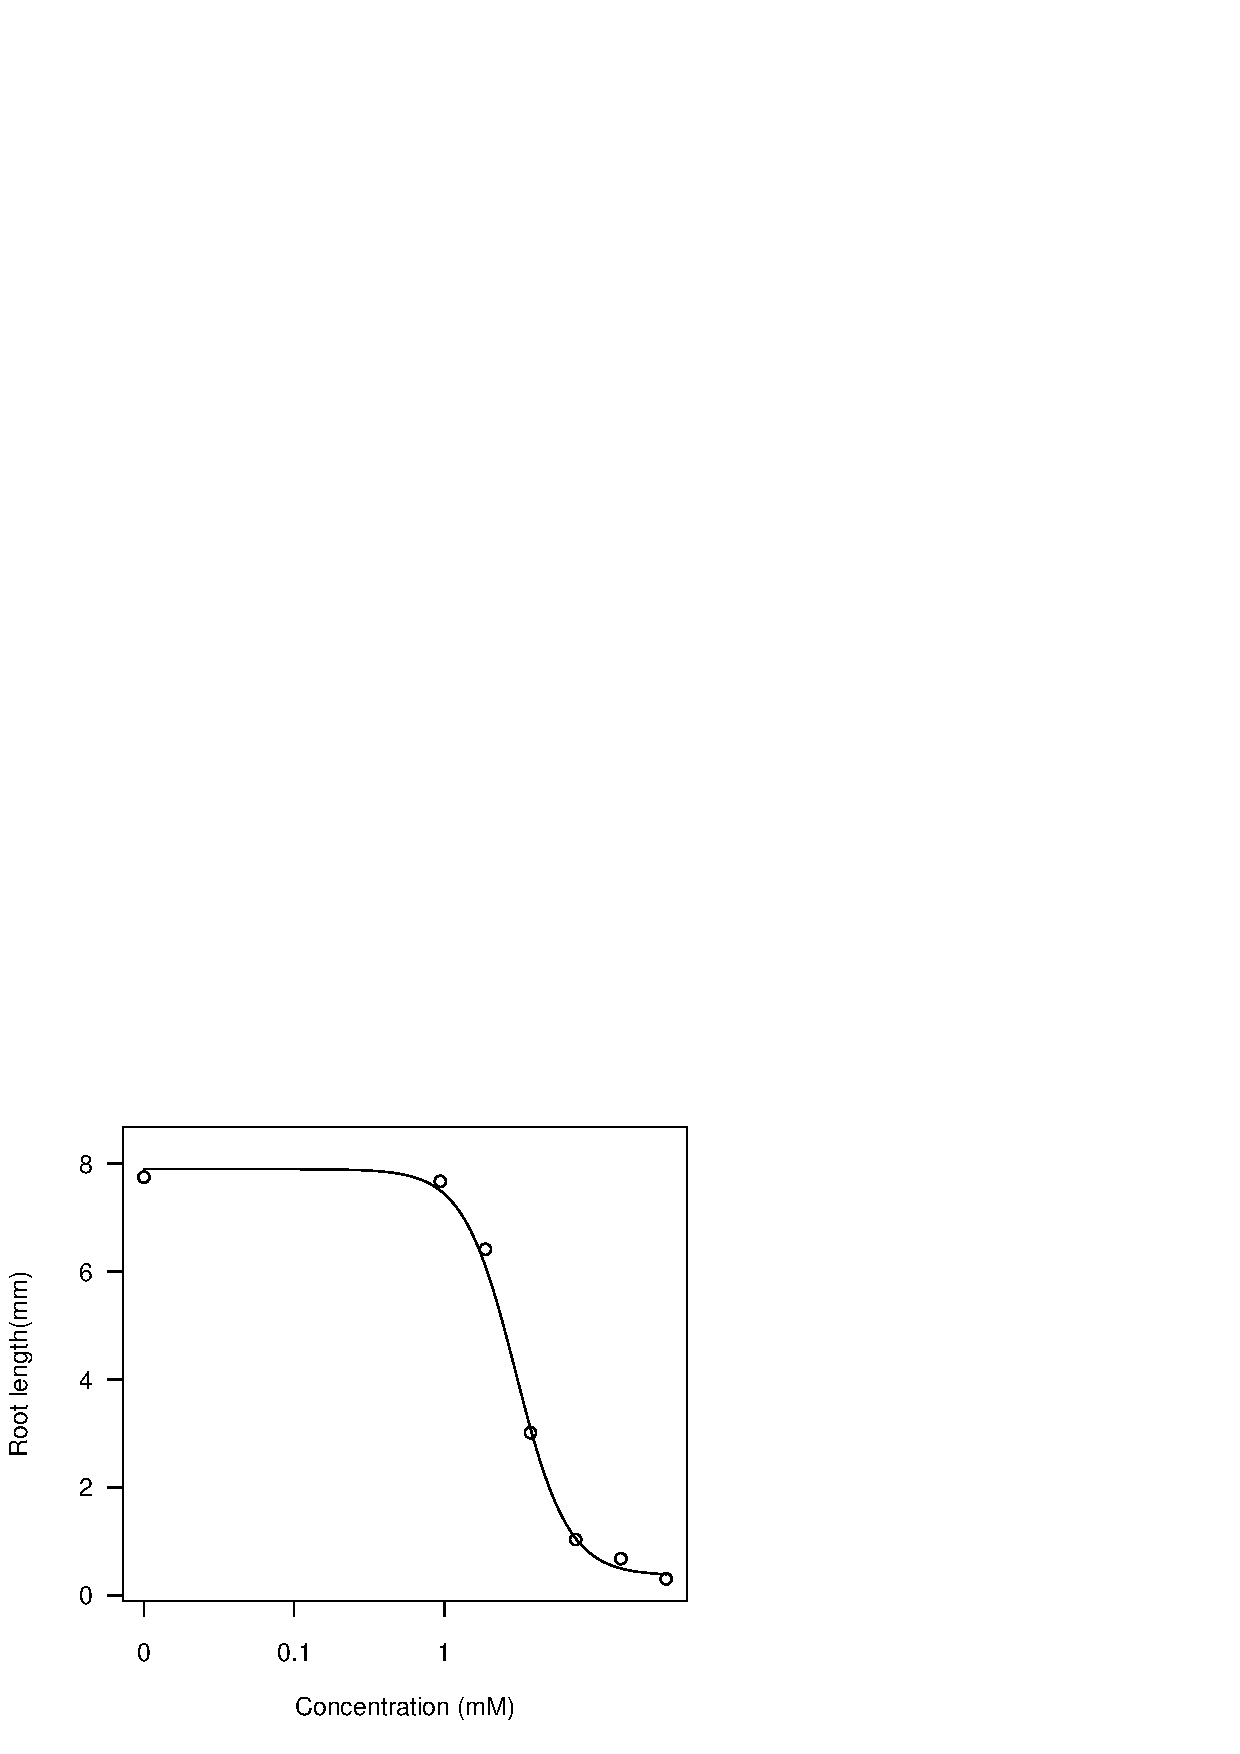
\includegraphics{drc-sec4-plot1}
\caption{Four-parameter logistic fit to the data set \texttt{FA}.} \label{fig-onefit:boxcox}
\end{center}
\end{figure}

%######################################################
%######################################################
%######################################################

\newpage
\section{Simultaneous fitting: Summarising the results} \label{sec:5}

The data set \verb+PestSci+ consists of 5 curves each with 7 doses and in 3 replications. The variables are \verb+CURVE+, \verb+DOSE+ and \verb+SLOPE+, 
containing the curve number, the dose values and the response values, respectively. The response is 
rate of change of Oxygen consumption of chloroplast membranes versus the dose of a herbicide. 
Relevant references are \citet{streibig&dayan&rimando&duke:1999, nielsen&ritz&streibig:2004}. To load the data set \verb+PestSci+ 
type \verb+data(PestSci)+.

To get an overview an initial plot of the data set is useful. The function \verb+plotraw+ plots the dose values against the response values with
different plot symbols for the different dose response curves (Figure~\ref{sec5-plot1}). The plot may help getting a first impression of the data,
in particular with respect to the ranges of dose values and the range of response values.

\begin{figure}[!htbp]
\begin{center}

\begin{Schunk}
\begin{Sinput}
> plotraw(SLOPE ~ DOSE, CURVE, data = PestSci, ylab = "Rate of Oxygen Evolutions", 
+     colour = TRUE)
\end{Sinput}
\end{Schunk}
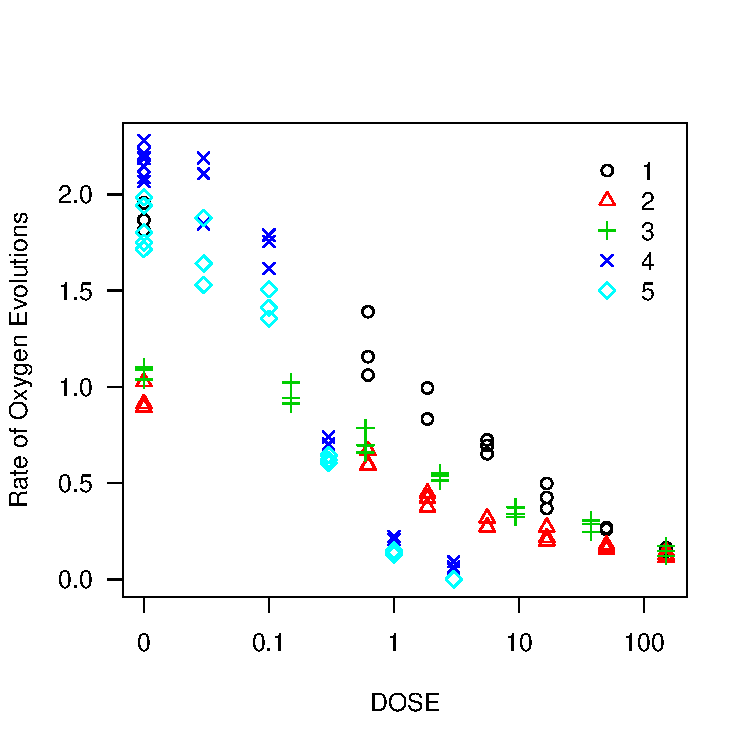
\includegraphics{drc-sec5-plot1}
\caption{Plot of the data in the data set \texttt{PestSci}.} \label{sec5-plot1}
\end{center}
\end{figure}

We consider simultaneous fitting of the 5 dose response curves in \verb+PestSci+, assuming each curve follows a four-parameter
logistic curve. Furthermore, we assume the parameters differ among curves (in total 4$\cdot$5=20 parameters).
This model is fitted using the \verb+multdrc+ function

\begin{Schunk}
\begin{Sinput}
> modelex2 <- multdrc(SLOPE ~ DOSE, CURVE, data = PestSci)
\end{Sinput}
\end{Schunk}
The formula \verb+SLOPE~DOSE+ in the first position relates response to dose. The variable \verb+CURVE+ in the second position is the grouping variable,
uniquely assigning each observation to a curve.
The argument \verb+data=PestSci+ specifies the data frame where the variables \verb+CURVE+, \verb+DOSE+ and \verb+SLOPE+ are found.

The lack-of-fit test comparing the simultaneous four-parameter logistic model to the alternative two-way ANOVA model is obtained applying the
function \verb+anova+ to the object \verb+modelex2+

\begin{Schunk}
\begin{Sinput}
> anova(modelex2)
\end{Sinput}
\begin{Soutput}
Lack-of-fit test

              ModelDf     RSS Df F value p value
Two-way ANOVA      70 0.38635                   
DRC model          85 0.45973 15  0.8863  0.5818
\end{Soutput}
\end{Schunk}
The test is not significant, meaning that the non-linear regression model provides an acceptable description of the data.
Subsequently, we proceed to look at the parameter estimates. The estimates and their standard errors are obtained using the function \verb+summary+

\begin{Schunk}
\begin{Sinput}
> summary(modelex2)
\end{Sinput}
\begin{Soutput}
A 'logistic' model was fitted.

Parameter estimates:

       Estimate  Std. Error     t-value   p-value
b:1  0.51954579  0.07637915  6.80219383 1.355e-09
b:2  0.80082699  0.22571773  3.54791357    0.0006
b:3  0.68200370  0.12858791  5.30379337 8.859e-07
b:4  1.84486652  0.16639052 11.08756974 1.714e-18
b:5  1.67107651  0.17602264  9.49353171 5.371e-15
c:1 -0.01656176  0.10784269 -0.15357332    0.8783
c:2  0.13259441  0.04720028  2.80918702    0.0062
c:3  0.14645523  0.06042448  2.42377301    0.0175
c:4  0.07955753  0.03946655  2.01582172    0.0470
c:5 -0.00092519  0.04340713 -0.02131434    0.9830
d:1  1.87954967  0.04237996 44.34996782 7.540e-61
d:2  0.94599411  0.04227580 22.37672971 1.101e-37
d:3  1.09032061  0.04056922 26.87556476 1.288e-43
d:4  2.15356998  0.02819071 76.39289139 2.051e-80
d:5  1.80502033  0.02909071 62.04800035 7.160e-73
e:1  1.79489240  0.47830988  3.75257230    0.0003
e:2  0.94558000  0.24956415  3.78892556    0.0003
e:3  1.37277472  0.45262844  3.03289542    0.0032
e:4  0.19732450  0.01019122 19.36220239 3.277e-33
e:5  0.20940785  0.01360994 15.38638612 1.352e-26

Estimated residual variance: 0.005408604 
\end{Soutput}
\end{Schunk}
From the summary it is seen that the lower limit of dose response curve no. 1 and no. 5 are negative which, strictly speaking, is not meaningful,
but these two lower limits are not significantly different from zero (right-most column). Comparison of parameters between curves can
be accomplished using the \verb+compParm+ function.

\newpage
A plot of the original observations and the fitted dose response curves is obtained using the \verb+plot+ function. The resulting plot is displayed
in Figure~\ref{sec5-plot2}, showing reasonable agreement between observations and fitted curves.

\begin{figure}[!htbp]
\begin{center}

\begin{Schunk}
\begin{Sinput}
> plot(modelex2, xlab = "Dose", ylab = "Rate of Oxygen Evolution", 
+     conName = "Control", col = TRUE)
\end{Sinput}
\end{Schunk}
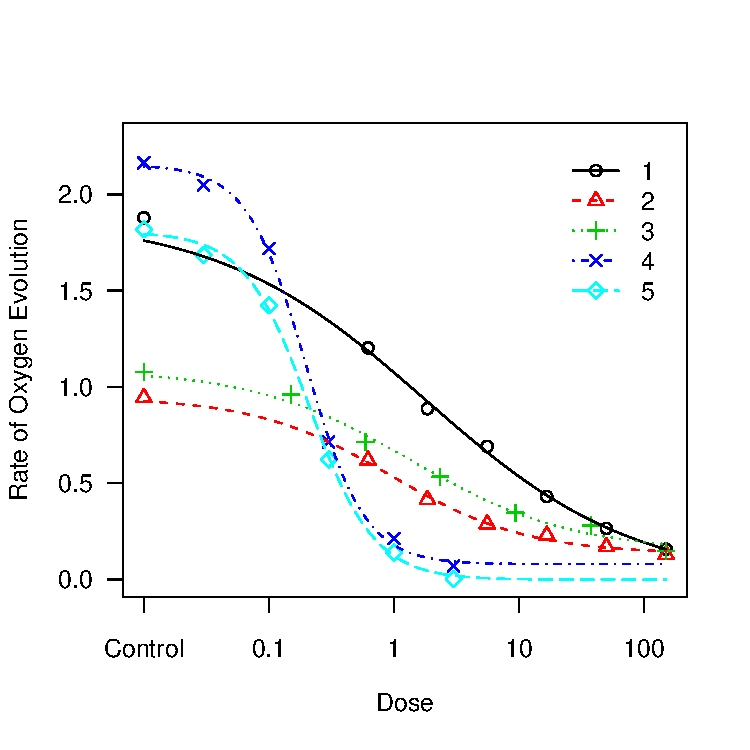
\includegraphics{drc-sec5-plot2}
\caption{Observed data and fitted dose response curves for the data set \texttt{PestSci}.} \label{sec5-plot2}
\end{center}
\end{figure}

The call \verb+plot(modelex2, obs="none")+ produces a similar plot,
but without the observations. Also the argument \verb+conName+ specifies the name of the tick mark for the dose level that can be considered as dose 0.
The usual graphical parameters in \textbf{R} can also be supplied in the function call; for instance \verb+xlab+
and \verb+ylab+ to change the default labels of the axes (which are the names of the variables in the data frame).
For more details on the \verb+plot+ function see \verb+?plot.drc+.

%\newpage
As already mentioned in Section~\ref{sec:2}, the package \verb+drc+  provides functions \verb+ED+ and \verb+SI+ to compute EDx values 
and selectivity indices SI(x,y), respectively, for the built-in models like the four-parameter logistic model. As an example we calculate 
estimates of the parameters ED10, ED50 and ED90 and their standard errors for all curves in \verb+PestSci+. The call to \verb+ED+ is

\begin{Schunk}
\begin{Sinput}
> ED(modelex2, c(10, 50, 90))
\end{Sinput}
\begin{Soutput}
       Estimate Std. Error
1:10   0.026143     0.0127
1:50   1.794892     0.4783
1:90 123.232283   101.6493
2:10   0.060831     0.0480
2:50   0.945580     0.2496
2:90  14.698386    12.4191
3:10   0.054755     0.0295
3:50   1.372775     0.4526
3:90  34.417098    28.0792
4:10   0.059971     0.0068
4:50   0.197325     0.0102
4:90   0.649267     0.0807
5:10   0.056229     0.0080
5:50   0.209408     0.0136
5:90   0.779880     0.1267
\end{Soutput}
\end{Schunk}
Notice that the estimates for the parameter ED50 already were displayed above in the \verb+summary+ output as the standard parameterization of the
four-parameter logistic model involves ED50.
The selectivity indices between two curves for ED10 and ED90, SI(90,10), are obtained using the call

\begin{Schunk}
\begin{Sinput}
> SI(modelex2, c(90, 10))
\end{Sinput}
\begin{Soutput}
            Estimate Std. Error    t-value   p-value
1/2:90/10 2025.80475 2311.43649    0.87599    0.3835
1/3:90/10 2250.60975 2216.78443    1.01481    0.3131
1/4:90/10 2054.87546 1711.04427    1.20036    0.2333
1/5:90/10 2191.62442 1834.71378    1.19399    0.2358
2/3:90/10  268.43884  268.93170    0.99445    0.3228
2/4:90/10  245.09286  208.95610    1.16815    0.2460
2/5:90/10  261.40343  224.00382    1.16250    0.2483
3/4:90/10  573.89873  472.75048    1.21184    0.2289
3/5:90/10  612.09085  506.97840    1.20536    0.2314
4/5:90/10   11.54688    2.18721    4.82207 6.166e-06
\end{Soutput}
\end{Schunk}
The output provides standard errors of the estimates and $p$-values for testing the null hypothesis that the indices are equal to 1. 

The use of SI is best illustrated by using the methods chemical
companies use to quantify selectivity in their research and
development of new herbicides. Since herbicides have an effect on
any plant, be it crops or weeds, we sometimes have to accept a
small decrease in the crop yield, for example a 10\% decrease
might be tolerated (ED10), while a 90\% control of the weed
(ED90) is considered a reasonable control level. The larger the
SI the more selective is one herbicide as compared to another herbicide. Obviously, the above SI(90,10) values are all much
larger than 1.00, but only for curve no 4 and 5 the value is significantly larger than 1.00.
\\
\\
The function \verb+SI+ can also be used to compare potencies among absolute
response levels. The EDx for a dose response curve is a relative response level depending upon
the upper and lower limits of the curve. For example in \verb+PestSci+ the response for the dose ED50 for the 2nd curve is
0.54 ((0.94+0.13)/2) whilst for the 4th curve the response level is 1.38 ((2.15+0.08)/2). In fact 1.38
exceeds the maximum response level of the 2nd curve. Consequently, we sometimes want to compare two curves
at a certain absolute response level and it can easily be done with \verb+SI+. Let us assume that
for various reasons we want to compare curves 2 and 4 at an absolute response level of 0.5. For the 2nd curve it means at the
dose ED46 ( 0.46 = (0.5-0.13)/(0.94-0.13) ) and for 4th curve at the dose ED21.
To obtain only the comparison between the 2nd curve and the 4th curve we use \verb+SI+ with an extra vector argument giving the curves to be compared

\begin{Schunk}
\begin{Sinput}
> SI(modelex2, c(46, 21), c(2, 4))
\end{Sinput}
\begin{Soutput}
          Estimate Std. Error t-value p-value
2/4:46/21   8.0438     2.2114  3.1853   0.002
\end{Soutput}
\end{Schunk}


%######################################################
%######################################################
%######################################################

\newpage
\section{Simultaneous fitting: Model reduction} \label{sec:6}

In this section we illustrate how to reduce a model using significance tests.
\\
\\
The data set \verb+TM+ comprises of 7 response curves, measured at a number of positive dose values, and an additional group of measurements at dose zero.
A separate control group frequently occurring case in bioassay analysis.
There are three variables: \verb+dose+ is the dose, \verb+pct+ the curve number and \verb+rgr+ the response.
The responses are growth rates of duckweed and the treatments are mixtures of two herbicides with different modes of action \citep{cedergreen:2004}. 
There are 180 observations.

We define a simultaneous model, assuming that each dose response curve follows a four-parameter Weibull model (\ref{w4})
and with different parameters for different assays. This model is specified as follows

\begin{Schunk}
\begin{Sinput}
> modelex3.1 <- multdrc(rgr ~ dose, pct, data = TM, fct = w4())
\end{Sinput}
\begin{Soutput}
Control measurements detected for level: 999
\end{Soutput}
\end{Schunk}
As \verb+pct+ take 8 different values (7 curves + control group), we are specifying a model with 8 curves, where the curve corresponding to the control
group only is defined as dose equal to 0 and thus not constitutes an entire dose response curve.
The asymmetric four-parameter Weibull model is specified with the argument \verb+fct=w4()+. 
The lack-of-fit test against the two-way ANOVA using \verb+anova+ (not displayed) confirms that the Weibull model fits the data.
\\
\\
A summary of the fit \verb+modelex3.1+ is

\begin{Schunk}
\begin{Sinput}
> summary(modelex3.1)
\end{Sinput}
\begin{Soutput}
A 'Weibull' model was fitted.

Parameter estimates:

         Estimate  Std. Error     t-value   p-value
b:100  1.0643e+00  2.1743e-01  4.8948e+00 2.501e-06
b:83   7.6661e-01  2.8917e-01  2.6511e+00    0.0089
b:67   7.8423e-01  1.5040e-01  5.2143e+00 5.980e-07
b:50   1.7377e+00  2.9132e-01  5.9651e+00 1.669e-08
b:33   8.0459e-01  1.4177e-01  5.6755e+00 6.864e-08
b:17   9.1325e-01  1.8109e-01  5.0431e+00 1.297e-06
b:0    1.1065e+00  2.0918e-01  5.2899e+00 4.227e-07
c:100  1.0908e-02  9.9819e-03  1.0928e+00    0.2762
c:83   2.8171e-04  3.2412e-02  8.6914e-03    0.9931
c:67  -8.8010e-03  1.4109e-02 -6.2380e-01    0.5337
c:50  -4.1308e-03  9.4332e-03 -4.3790e-01    0.6621
c:33  -1.8937e-02  1.2262e-02 -1.5444e+00    0.1246
c:17  -3.9700e-03  1.1849e-02 -3.3503e-01    0.7381
c:0   -9.8622e-03  9.5501e-03 -1.0327e+00    0.3034
d:999  2.8149e-01  6.8316e-03  4.1205e+01 2.460e-84
d:100  3.4991e-01  2.4662e-02  1.4189e+01 7.068e-30
d:83   3.3115e-01  3.8113e-02  8.6887e+00 5.593e-15
d:67   3.6687e-01  3.1103e-02  1.1795e+01 1.796e-23
d:50   2.7986e-01  1.0346e-02  2.7051e+01 4.488e-60
d:33   3.7504e-01  3.1746e-02  1.1814e+01 1.603e-23
d:17   3.3019e-01  2.5505e-02  1.2946e+01 1.464e-26
d:0    3.0591e-01  2.1229e-02  1.4410e+01 1.833e-30
e:100  1.3059e+02  1.4770e+01  8.8415e+00 2.257e-15
e:83   2.8364e+03  6.5786e+02  4.3115e+00 2.914e-05
e:67   3.9831e+03  6.1822e+02  6.4428e+00 1.485e-09
e:50   7.4642e+03  6.0733e+02  1.2290e+01 8.422e-25
e:33   6.9756e+03  1.0298e+03  6.7738e+00 2.624e-10
e:17   8.8374e+03  1.2141e+03  7.2786e+00 1.721e-11
e:0    1.0201e+04  1.1720e+03  8.7036e+00 5.135e-15

Estimated residual variance: 0.0005600451 
\end{Soutput}
\end{Schunk}
By default only the $d$ parameter (the upper limit at dose zero) is estimated for the control group, represented in the summary by the term \verb+d:999+.

%\newpage
Figure~\ref{sec6-plot1} clearly shows that allowing individual upper limits for the individual curves does not produce a fit that agrees with the
control group.

\begin{figure}[!htbp]
\begin{center}
\begin{Schunk}
\begin{Sinput}
> plot(modelex3.1, ylim = c(-0.05, 0.4), conLevel = 1)
\end{Sinput}
\end{Schunk}
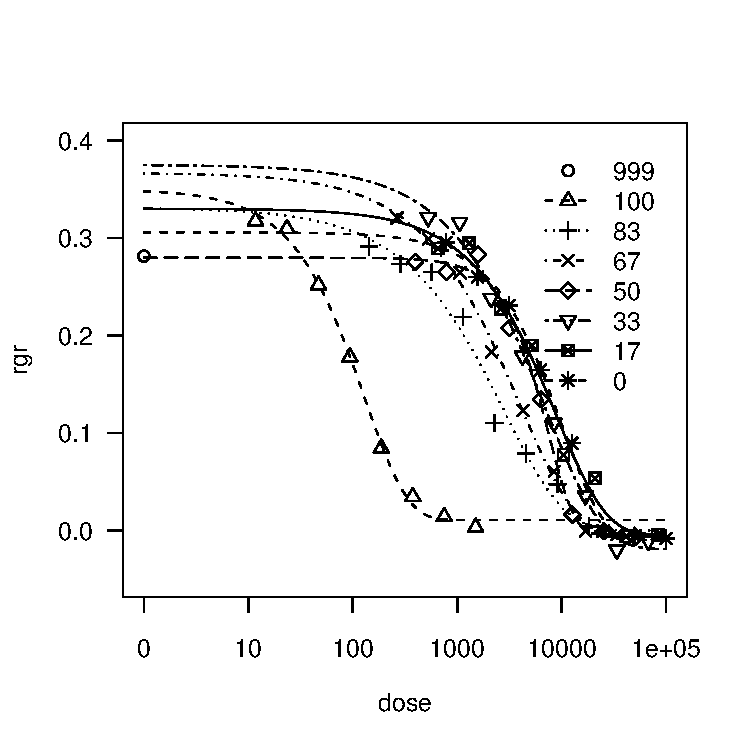
\includegraphics{drc-sec6-plot1}
\caption{Observed data and fitted dose response curves for the data set \texttt{TM}.} \label{sec6-plot1}
\end{center}
\end{figure}

A more reasonable initial model would only have a single $d$ parameter common to all curves, as the control group determines the common upper limit for
all 7 curves.
This can be specified in \verb+multdrc+ using the \verb+collapse+ argument specifying which parameters should be collapsed across assays. 
This argument may be
specified using a data frame or a list as argument. If no \verb+collapse+ argument is given there are different parameters for different curves
(used in sections~\ref{sec:4} and~\ref{sec:5}).
The two types of argument are overlapping in their functionality, but not entirely identical, both have strong points.
The data frame specification is better for collapsing parameters for arbitrary curves, without requiring the corresponding grouping variable to be defined.
The list specification allows more general structures involving more than one variable per parameter. Specification of the 
\verb+collapse+ argument by means of a list of formulas, follows the same syntax as is used for \verb+lm+ and \verb+glm+.

The data frame should contain as many columns as there are parameters in the model, eg four columns in case of the four-parameter Weibull model, 
and the columns correspond to parameters by order, eg the first column
corresponds to $b$, $\ldots$, the fourth column to $e$. For built-in function the order of parameters is always alphabetical. 
Observations sharing the same value in a column will share the corresponding parameter in the model. We specify the model with common upper as follows

\begin{verbatim}
modelex3.2<-multdrc(TM[,c(3,1)], TM[,2],
collapse=data.frame(TM[,2], TM[,2], colFct(TM[,2],1:8), TM[,2]), fct=w4())
\end{verbatim}
\begin{Schunk}
\begin{Soutput}
Control measurements detected for level: 999
\end{Soutput}
\end{Schunk}

The column \verb+TM[,2]+ contains the values enumerating the different curves (180 values)

\begin{Schunk}
\begin{Soutput}
  [1] 999 999 999 999 999 999 999 999 999 999 999 999 100 100 100 100 100 100
 [19] 100 100 100 100 100 100 100 100 100 100 100 100 100 100 100 100 100 100
 [37]  83  83  83  83  83  83  83  83  83  83  83  83  83  83  83  83  83  83
 [55]  83  83  83  83  83  83  67  67  67  67  67  67  67  67  67  67  67  67
 [73]  67  67  67  67  67  67  67  67  67  67  67  67  50  50  50  50  50  50
 [91]  50  50  50  50  50  50  50  50  50  50  50  50  50  50  50  50  50  50
[109]  33  33  33  33  33  33  33  33  33  33  33  33  33  33  33  33  33  33
[127]  33  33  33  33  33  33  17  17  17  17  17  17  17  17  17  17  17  17
[145]  17  17  17  17  17  17  17  17  17  17  17  17   0   0   0   0   0   0
[163]   0   0   0   0   0   0   0   0   0   0   0   0   0   0   0   0   0   0
\end{Soutput}
\end{Schunk}
Thus in \verb+modelex3.2+ the parameters $b$, $c$ and $e$ will vary from curve to curve. The function \verb+colFct+ is used for
collapsing a column into a column with fewer distinct values. The call \verb+colFct(TM[,3], 1:8)+ collapses all 8 different values in \verb+TM[,2]+ into 
a single value. The content of \verb+colFct(TM[,2], 1:8)+ is (again 180 values)

\begin{Schunk}
\begin{Soutput}
  [1] 1 1 1 1 1 1 1 1 1 1 1 1 1 1 1 1 1 1 1 1 1 1 1 1 1 1 1 1 1 1 1 1 1 1 1 1 1
 [38] 1 1 1 1 1 1 1 1 1 1 1 1 1 1 1 1 1 1 1 1 1 1 1 1 1 1 1 1 1 1 1 1 1 1 1 1 1
 [75] 1 1 1 1 1 1 1 1 1 1 1 1 1 1 1 1 1 1 1 1 1 1 1 1 1 1 1 1 1 1 1 1 1 1 1 1 1
[112] 1 1 1 1 1 1 1 1 1 1 1 1 1 1 1 1 1 1 1 1 1 1 1 1 1 1 1 1 1 1 1 1 1 1 1 1 1
[149] 1 1 1 1 1 1 1 1 1 1 1 1 1 1 1 1 1 1 1 1 1 1 1 1 1 1 1 1 1 1 1 1
\end{Soutput}
\end{Schunk}
Therefore this column results in a single common $d$ parameter for all assays.
\\
\\
The above model can also be specified using the names of the variables in \verb+TM+ and using the constant factor. Thus
the alternative specification looks like

\begin{verbatim}
modelex3.2 <- multdrc(rgr~dose, pct, collapse=data.frame(pct, pct, 1, pct),
data=TM, fct=w4())
\end{verbatim}
or, using a list

\begin{verbatim}
modelex3.2 <- multdrc(rgr~dose, pct, 
collapse=list(~factor(pct), ~factor(pct), ~1, ~factor(pct)),
data=TM, fct=w4())
\end{verbatim}
In order to compare \verb+modelex3.2+ to \verb+modelex3.1+ the \verb+anova+ function can be used.
The \verb+anova+ function with the two model objects as arguments produces an approximate F-test (or a likelihood ratio test) for test of reduction 
of the
larger model to the smaller model. For the models \verb+modelex3.1+ and \verb+modelex3.2+ \verb+anova+ gives an F-test for reduction from the model
with different upper limits to the model with a common upper limit.

\begin{Schunk}
\begin{Sinput}
> anova(modelex3.1, modelex3.2)
\end{Sinput}
\begin{Soutput}
1st model
 fct:      w4()
 collapse: pct (for all parameters)
2nd model
 fct:      w4()
 collapse: TM[, 2], TM[, 2], colFct(TM[, 2], 1:8), TM[, 2]

ANOVA table

          ModelDf      RSS  Df F value   p value
2nd model     158 0.109028                      
1st model     151 0.084567   7  6.2397 1.969e-06
\end{Soutput}
\end{Schunk}
The test is highly significant and the model with common upper limit is rejected. Notice that the order of the two arguments in \verb+anova+ does not matter.
The main problem with the data set \verb+TM+ is the presence of hormesis (described in section~\ref{sec:5}), thus a more appropriate approach 
would be to use a hormesis model \citep{cedergreen&ritz&streibig:2005}.
\\
\\
Another aspect of \verb+modelex3.1+ is that it seems from the summary of \verb+modelex3.1+ that all lower limits are equal. The model with a common lower limit is

\begin{Schunk}
\begin{Sinput}
> modelex3.3 <- multdrc(rgr ~ dose, pct, collapse = data.frame(pct, 
+     1, pct, pct), data = TM, fct = w4())
\end{Sinput}
\begin{Soutput}
Control measurements detected for level: 999
\end{Soutput}
\end{Schunk}
The test for model reduction is not significant

\begin{Schunk}
\begin{Sinput}
> anova(modelex3.3, modelex3.1)
\end{Sinput}
\begin{Soutput}
1st model
 fct:      w4()
 collapse: pct, 1, pct, pct
2nd model
 fct:      w4()
 collapse: pct (for all parameters)

ANOVA table

          ModelDf      RSS  Df F value p value
1st model     157 0.087083                    
2nd model     151 0.084567   6  0.7487  0.6114
\end{Soutput}
\end{Schunk}
Thus \verb+modelex3.3+ provides as good a fit to the data as does \verb+modelex3.1+. Next we fit a model with the common lower limit equal to 0. This
can be done using the built-in function \verb+w3()+ which is a three-parameter Weibull model (lower limit set to 0).

\begin{Schunk}
\begin{Sinput}
> modelex3.4 <- multdrc(rgr ~ dose, pct, data.frame(pct, pct, pct), 
+     data = TM, fct = w3())
\end{Sinput}
\begin{Soutput}
Control measurements detected for level: 999
\end{Soutput}
\end{Schunk}
The F-test for reduction from \verb+modelex3.3+ to \verb+modelex3.4+ is

\begin{Schunk}
\begin{Sinput}
> anova(modelex3.4, modelex3.3)
\end{Sinput}
\begin{Soutput}
1st model
 fct:      w3()
 collapse: pct, pct, pct
2nd model
 fct:      w4()
 collapse: pct, 1, pct, pct

ANOVA table

          ModelDf      RSS  Df F value p value
1st model     158 0.087804                    
2nd model     157 0.087083   1  1.2997  0.2560
\end{Soutput}
\end{Schunk}
Thus we can reduce the initial model to a model with common lower limit equal to 0.

%######################################################
%######################################################
%######################################################

\newpage
\section{A user-defined function} \label{sec:7}

Consider the data set \verb+Puromycin+ available in \textbf{R}. In the help page \verb+?Puromycin+, a Michaelis-Menten model is suggested. 
This model has the form

\begin{equation} \label{MM}
y = f \big( x, (Vm, K) \big) = \frac{Vm x}{K + x}
\end{equation}
with two parameters, \emph{Vm} and \emph{K}. Define this non-linear function in \textbf{R} as follows

\begin{Schunk}
\begin{Sinput}
> MMfct <- function(x, parm) {
+     parm[, 1] * x/(parm[, 2] + x)
+ }
\end{Sinput}
\end{Schunk}
where \verb+parm+ is matrix consisting of two columns: \verb+parm[,1]+ and \verb+parm[,2]+ corresponding to \emph{Vm} and \emph{K}, respectively. 
A self starter function could be defined taking the maximum of the response values as initial estimate of \emph{Vm} and, using this initial estimate of
\emph{Vm}, the equation~(\ref{MM}) is then solved in \emph{K} for an arbitrary pair $(x, y)$ (we take the first pair in the data set). Thus the self starter
function looks like

\begin{Schunk}
\begin{Sinput}
> MMssfct <- function(data) {
+     Vm <- max(data[, 2])
+     K <- Vm * data[1, 1]/(data[1, 2] - data[1, 1])
+     return(c(Vm, K))
+ }
\end{Sinput}
\end{Schunk}
where \verb+data+ is a data frame containing $x$ values in the first column and $y$ values in the second column. Finally we set the names of
the parameters (\emph{Vm} and \emph{K})

\begin{Schunk}
\begin{Sinput}
> MMnames <- c("Vm", "K")
\end{Sinput}
\end{Schunk}
Now we are ready to use the function \verb+multdrc+. Fitting a simultaneous Michaelis-Menten model to the two states is accomplished using the call

\begin{Schunk}
\begin{Sinput}
> modelex4 <- multdrc(rate ~ conc, state, data = Puromycin, fct = list(MMfct, 
+     MMssfct, MMnames))
\end{Sinput}
\end{Schunk}
A summary of the model fit containing parameter estimates and estimated standard errors and a comparison of the two $Vm$ parameters is given below.

\begin{Schunk}
\begin{Sinput}
> summary(modelex4)
\end{Sinput}
\begin{Soutput}
A 'drc' model was fitted.

Parameter estimates:

               Estimate Std. Error    t-value   p-value
Vm:treated   2.1268e+02 6.8100e+00 3.1231e+01 4.275e-18
Vm:untreated 1.6028e+02 7.2403e+00 2.2137e+01 4.938e-15
K:treated    6.4121e-02 8.2832e-03 7.7411e+00 2.722e-07
K:untreated  4.7708e-02 8.9551e-03 5.3275e+00 3.846e-05

Estimated residual variance: 108.1607 
\end{Soutput}
\end{Schunk}
A comparison of the difference between the two \emph{Vm} parameters is obtained using the \verb+compParm+ function
\begin{Schunk}
\begin{Sinput}
> compParm(modelex4, "Vm", "-")
\end{Sinput}
\begin{Soutput}
Comparison of parameter 'Vm' 

                  Estimate Std. Error t-value   p-value
treated-untreated  52.4038     9.9397  5.2722 4.344e-05
\end{Soutput}
\end{Schunk}


%######################################################
%######################################################
%######################################################

%\newpage
%\section{An additive model} \label{sec:8}

%The data set \verb+PestSci2+ consists of 4 dose response curves. Dose values and response values are denoted \verb+DOSE+ and \verb+SLOPE+,
%respectively.
%The grouping variable is \verb+CURVE+ and in addition there are two two-level factors \verb+A+ (levels: \verb+a+, \verb+b+) and \verb+B+
%(levels: \verb+1+, \verb+2+), measured for each observation.
%We assume a four-parameter logistic model. 
%A model with an additive model of the form \verb!A+B! for the parameter $d$ and interaction structure (\verb+A:B+) for the remaining parameters 
%can be specified using a list of formulas
%
%<<sec8-fit2, echo=F>>=
%
%modelex5.1 <- multdrc(SLOPE~DOSE, CURVE, collapse=list(~A*B, ~A*B, ~A+B, ~A*B), data=PestSci2)
%
%@
%\begin{verbatim}
%modelex5.1 <- multdrc(SLOPE~DOSE, CURVE, 
%collapse=list(~A*B, ~A*B, ~A+B, ~A*B),
%data=PestSci2)
%\end{verbatim}
%A summary of the fit is
%
%<<sec8-summary, echo=T>>=
%
%summary(modelex5.1)
%
%@ 


\newpage
\section{Conclusions} \label{sec:conclusions}

We have described the package \verb+drc+ for fitting multiple non-linear regression models, with special focus on applications in bioassay analysis. 
Thus the package \verb+drc+ is an attempt to develop a collection of functions specifically designed for bioassay analysis. Relevant interpretations 
of a model fit is easy using the built-in models.

At the same time we would like to emphasize that \verb+drc+ provides functionality for simultaneous fitting of arbitrary non-linear regression models
under the assumption of independent and normally distributed measurement errors, such functionality was not previously available in \textbf{R}.

%\section*{Acknowledgement}
%We are grateful to Oscar Go for working his way through an earlier version of the paper and detecting several errors.

%\newpage
\bibliographystyle{sjs}
\bibliography{c:/stat/projects/bioassay/bioassay}

\end{document}
